\documentclass[review]{elsarticle}

\journal{Annals of Nuclear Energy}
%%%% packages and definitions (optional)
\newcommand{\Cyclus}{\textsc{Cyclus}\xspace}%
\newcommand{\Cycamore}{\textsc{Cycamore}\xspace}

\usepackage{lineno}
\usepackage{tabularx}
\usepackage[acronym,toc]{glossaries}
\include{acros}
\makeglossaries
\usepackage{xspace}

\usepackage{caption}
\newcolumntype{b}{X}
\newcolumntype{s}{>{\hsize=.5\hsize}X}
\newcolumntype{m}{>{\hsize=.75\hsize}X}



\usepackage{tikz}
\usetikzlibrary{shapes.geometric,arrows}
\tikzstyle{process} = [rectangle, rounded corners, minimum width=3cm, minimum height=1cm,text centered, draw=black, fill=blue!30]
\tikzstyle{object} = [ellipse, rounded corners, minimum width=3cm, minimum height=1cm,text centered, draw=black, fill=green!30]
\tikzstyle{arrow} = [thick,->,>=stealth]
\usetikzlibrary{positioning, arrows, decorations, shapes }%


\begin{document}

\begin{frontmatter}
\title{Standardized Verification of the Cyclus Fuel Cycle Simulator}
\author{Jin Whan Bae$^{1}$, Joshua L. Peterson-Droogh$^{2}$, Kathryn D. Huff$^{1}$}
\address{$^{1}$Dept. of Nuclear, Plasma, and Radiological Engineering, University of Illinois at Urbana-Champaign, Urbana, IL \\ $^{2}$Oak Ridge National Laboratory, Oak Ridge, TN }

\begin{abstract}
Many nuclear fuel cycle simulators can analyze transitions from once-through to 
advanced nuclear fuel cycles. Verification studies compare various fuel 
cycle analysis tools to test agreement and identify sources of difference.  A 
recent verification study, B. Feng et al., ``Standardized verification of fuel 
cycle modeling,'' Annals of Nuclear Energy, vol. 94, pp. 300-312, Aug.  2016 
\cite{feng_standardized_2016} established transition scenario test case 
specifications and accordingly evaluated national laboratory nuclear fuel cycle 
simulators, DYMOND, VISION, ORION, and  MARKAL.  This work verifies the 
performance of \Cyclus, the agent-based, open-source fuel cycle simulator, 
using the test case specifications in Feng et. al.  In this work, \Cyclus 
demonstrates agreement with the results from the previous verification study. 
Minor differences reflect intentional, detailed material tracking in the 
\Cycamore reactor module.  These results extend the example results in Feng et. 
al to further enable future verification of additional nuclear fuel cycle 
simulation tools.  
\end{abstract}


\end{frontmatter}

\modulolinenumbers[5]
\linenumbers
	
\section{Abstract}
Numerous nuclear fuel cycle system modeling codes
have been developed to perform fuel cycle transition
analyses from a once-through cycle to an advanced
fuel cycle. Verification studies compare different
fuel cycle analysis tools against each other to
test agreement and identify sources of difference.
This paper benchmarks \Cyclus, the agent-based,
open-source fuel cycle simulation code, against
a verification study \cite{feng_standardized_2016} with
DYMOND \cite{yacout_2005_modeling},
VISION \cite{jacobson_2010_verifiable},
ORION \cite{gregg_2012_analysis}, and
MARKAL \cite{shay_2006_epa}. The study reveals
that \Cyclus' results match the spreadsheet results
very closely, with a minor difference with regard to
reprocessing \gls{UNF}. This difference is most
likely caused by two factors:
[GOOD WAY TO EXPLAIN]

\section{Introduction}
Fuel cycle simulators act as an important tool to
aid decision in policy and fuel cycle strategies.
To meet this need from various institutions, a
multitude of fuel cycle simulators were developed,
using different methods and different structures
to simulate the material flow in the nuclear fuel cycle.
The difference in the algorithm of fuel cycle analysis
codes combined with a small user community make
validation studies necessary to gain
confidence of the capability of the code as well as its
agreement with other analysis codes.

This study is done to benchmark \Cyclus' results
against that of other well-known codes, such as
DYMOND \cite{yacout_2005_modeling},
VISION \cite{jacobson_2010_verifiable},
ORION \cite{gregg_2012_analysis}, and
MARKAL \cite{shay_2006_epa}. We take the input
parameters and results from a validation study
\cite{feng_standardized_2016} already done for the
mentioned tools for a transition scenario from an
open fuel cycle to an advanced fuel cycle with
reprocessing. In the paper, the `model solutions'
generated from an excel worksheet are compared
with each code results, and the results show
excellent agreement.


\subsection{\Cyclus}

\Cyclus is an agent-based fuel cycle simulation framework 
\cite{huff_fundamental_2016}, which means 
that each reactor, reprocessing plant, and fuel fabrication plant is modeled as an agent.
A \Cyclus simulation contains prototypes, which are fuel cycle facilities with
pre-defined parameters, that are deployed in the simulation as \texttt{facility} agents.
Encapsulating the \texttt{facility} agents are the \texttt{Institution} and \texttt{Region}.
A \texttt{Region} agent holds a set of \texttt{Institution}s.
An \texttt{Institution} agent can deploy or decommission \texttt{facility} agents.
The \texttt{Institution} agent is part of a \texttt{Region} agent,
which can contain multiple \texttt{Institution} agents. Several versions of \texttt{Institution}
and \texttt{Region} exist, varying in complexity and functions \cite{huff_extensions_2014}.
 \texttt{DeployInst} is used as the institution archetype for this work, where the institution
deploys agents at user-defined timesteps.

At each timestep (one month),
agents make requests for materials or bid to supply them and exchange
with one another. A market-like mechanism called the dynamic resource exchange
\cite{gidden_agent-based_2015} governs the exchanges.
Each material resource has a quantity, composition, name, and a unique identifier
for output analysis. The timestep execution in \Cyclus follows 
\texttt{Build, Tick, \gls{DRE}, Tock, and Decommission}, as illustrated in
figure \ref{fig:time}. The \texttt{Tick}, and \texttt{Tock} phases are for
each agent to perform actions, such as transmutation, separation, generation,
of materials before and after the market exchange phase. 

\begin{figure}[h]
\centering
\scalebox{0.7}{
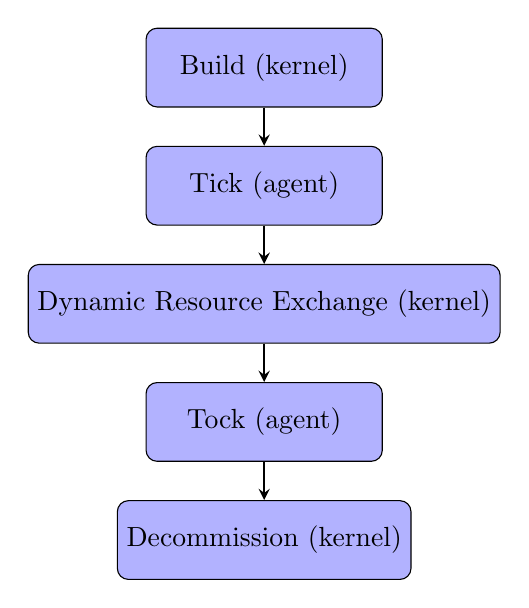
\begin{tikzpicture}[node distance=1.5cm]
\node (Build) [process] {Build (kernel)};
\node (Tick) [process, below of=Build] {Tick (agent)};
\node (DRE) [process, below of=Tick]{Dynamic Resource Exchange (kernel) };
\node (Tock) [process, below of=DRE]{Tock (agent)};
\node (Decom) [process, below of=Tock] {Decommission (kernel)};

\draw [arrow] (Build) -- (Tick); 
\draw [arrow] (Tick) -- (DRE);
\draw [arrow] (DRE) -- (Tock);
\draw [arrow] (Tock) -- (Decom);
\end{tikzpicture}
}
\caption{\Cyclus timestep execution steps.}
\label{fig:time}
\end{figure}

The modularity of \Cyclus allows a low barrier of
entry for developers, since developers can create an
archetype (e.g. Reactor module, Reprocessing module)
without extensive knowledge of the \Cyclus framework.

\section{Methodology}

Feng et al. comprehensively defines simulation parameters
sufficient to reproduce the transition scenario in \Cyclus.
In this study, we used the \Cycamore \cite{huff_fundamental_2016}
 archetype library to model
all fuel cycle facilities. \Cycamore libraries contain
simple fuel cycle facility models. 

The \Cyclus input file and analysis procedures are all
openly available in \cite{bae_arfc/transition-scenarios:_2018}.
\Cyclus results are output in either \texttt{.sqlite} or
\texttt{.h5} format. In this study, we used the
\texttt{.sqlite} format and analyzed the results
using a python script. We then compared the post-processed
output data to the results with the
model solution from the verification study \cite{feng_standardized_2016}.

The analysis and benchmark were performed iteratively,
where we improve the original result by communicating
with the authors of the benchmark. 
We analyzed the reasons for the differences from the original
result. Only one adjustment to the default reactor depletion modeling behavior 
was needed, regarding fuel handling upon reactor decommissioning.
Major differences in the facility behavior algorithms did not require 
adjustment. All model heuristics contributing to minor deviations from the 
benchmark are explained in detail.



\section{Fundamental Code Differences in \Cyclus}
There fundamental differences in \Cyclus that yields
different results from the paper. The `model solution'
in the paper is generated using an excel worksheet.
The model solution is acquired through personal contact
from the paper's author, Bo Feng of Argonne National
Laboratory.
\section{Results}

In the comparison visualizations, we represent each \Cyclus result as a solid 
line and each benchmark model solution as a dotted line. We obtained the benchmark 
model solutions through personal contact with benchmark author Bo Feng at Argonne 
National Laboratory.

Figure \ref{fig:pow_plot} shows the deployed reactor capacity, and
figure \ref{fig:dep} shows the \gls{LWR} retirement and \gls{SFR}
deployment. These figures are merely a comparison df
input data, showing that the scenarios are defined equivalently for
\Cyclus and the benchmark. 

\begin{figure}[htbp!]
    \begin{center}
        \includegraphics[scale=0.5]{./images/results_18/power_plot.png}
    \end{center}
        \caption{Deployed reactor capacities at the end of each year.}
    \label{fig:pow_plot}
\end{figure}


\begin{figure}[htbp!]
	\begin{center}
		\includegraphics[scale=0.5]{./images/results_18/dep.png}
	\end{center}
        \caption{\glspl{LWR} retired and \glspl{SFR} started up each year.}
	\label{fig:dep}
\end{figure}

Figure \ref{fig:fuel_load} shows the annual fuel loading rate.
The initial fuel loading for 100 \gls{LWR} reactors matches
the plot in the verification
study results. The oscillations caused by the 18 month refueling period
were aggregated into 12 month groups. As a result, the total fuel loaded
are equal for both plots.

Although indistinguishable visibly in figure \ref{fig:fuel_load}, \gls{SFR} fuel 
loading in the \Cyclus simulation differs by a small amount proportional
to the core mass difference mentioned in the previous section, due to fractional 
numbers of batches. Specifically:

\begin{align*} 
        \frac{\Delta m(t)}{\Delta M_{core}} & = N_{SFR}(t)\\ 
        \intertext{where}
        N_{SFR}(t) &= \text{Number of SFRs deployed at time t}\\
        m(t) &= \text{SFR fuel loading at time t}  \\
        \Delta m(t) &= m_{c}(t) - m_{b}(t)\\
        m_c(t) &= \mbox{SFR fuel batch mass loaded (\Cyclus)}\\
        m_b(t) &= \mbox{SFR fuel batch mass loaded (benchmark)}\\
        \Delta M_{core} &= M_c - M_b \\
        M_c &= \mbox{Total SFR core mass (\Cyclus)}\\ 
                &= 15.8 [tHM]\\
        M_b &= \mbox{Total SFR core mass (benchmark)}\\ 
                &= 15.63 [tHM].
\end{align*}

Figure \ref{fig:fuel_load_diff_norm} shows the
differences normalized by the core mass differences, overlaid on the
\gls{SFR} deployment. This shows that the differences only occur during
deployment due to the difference in core mass.

\begin{figure}[htbp!]
    \begin{center}
        \includegraphics[scale=0.5]{./images/results_18/fuel_load.png}
    \end{center}
        \caption{Annual fresh fuel loading rates (first cores and reload fuel).}
    \label{fig:fuel_load}
\end{figure}

\begin{figure}[htbp!]
    \begin{center}
        \includegraphics[scale=0.5]{./images/results_18/fuel_load_diff_norm.png}
    \end{center}
        \caption{Difference between annual fresh \gls{SFR} fuel loading rates (Cyclus - Benchmark) normalized by the core mass difference of an \gls{SFR} due to fractional batch size.}
    \label{fig:fuel_load_diff_norm}
\end{figure}


Figure \ref{fig:fuel_discharge_monthly} shows the inventory of discharged
\gls{UNF} in the mandatory cooling stage (four years for \gls{LWR}, one year for \gls{SFR}).
It also oscillates between the benchmark's
solution and converges, caused by the influx and the outflux of \gls{UNF}
into and out of the storage facility.
The \gls{SFR} inventory and fuel loading
solutions exactly match the benchmark solutions, minus the small ($1.07\%$) difference due to core
size.

Figure \ref{fig:waiting_monthly} shows the amount of cooled \gls{UNF} waiting for
reprocessing. The value is calculated by subtracting the cumulative difference between
the cooled inventory and the \gls{UNF} reprocessing throughput.
The visible oscillation shows the inventory in the storage facility 
before (high) and after (low) it sends that inventory for reprocessing.

\begin{figure}[htbp!]
    \begin{center}
        \includegraphics[scale=0.5]{./images/results_18/fuel_discharge_monthly.png}
    \end{center}
        \caption{Inventory of discharged \gls{UNF} in mandatory cooling storage.}
    \label{fig:fuel_discharge_monthly}
\end{figure}


\begin{figure}[htbp!]
    \begin{center}
        \includegraphics[scale=0.5]{./images/results_18/waiting_monthly.png}
    \end{center}
        \caption{Inventory of discharged and cooled \gls{UNF} waiting for reprocessing.}
    \label{fig:waiting_monthly}
\end{figure}


Figure \ref{fig:rep} shows the reprocessing throughput, which oscillates around
the benchmark solution. No oscillation exists in the beginning because the
\gls{LWR} \gls{UNF} reprocessing plant throughput peaks at 2,000 tons per year.

\begin{figure}[htbp!]
    \begin{center}
        \includegraphics[scale=0.5]{./images/results_18/rep.png}
    \end{center}
        \caption{Annual reprocessing throughputs.}
    \label{fig:rep}
\end{figure}


Figure \ref{fig:tru} shows the inventory of unused \gls{TRU} recovered from \gls{UNF}.
The \Cyclus results follow the benchmark solutions closely. However,
the larger \gls{SFR} core size causes \Cyclus results to be smaller than the benchmark results,
since more \gls{TRU} is used to
start up the newly deployed \glspl{SFR}. The difference decreases as the
\glspl{SFR} decommission, discharging more \gls{UNF} (and hence \gls{TRU}) than
the benchmark.

\begin{figure}[htbp!]
	\begin{center}
		\includegraphics[scale=0.5]{./images/results_18/tru.png}
	\end{center}
        \caption{Inventory of unused \gls{TRU} recovered from \gls{UNF}.}
	\label{fig:tru}
\end{figure}


\section{Discussion}

We benchmarked \Cyclus, the agent-based
fuel cycle simulator with results from another
verification study and saw good agreement
in a transition scenario.

Throughout this work, two major differences were identified
that led to the deviation
of \Cyclus results to that of the excel sheet. First,
the \Cycamore reactor depletes only half of its core
when decommissioned. Second, \Cyclus, unlike other
codes examined in the benchmark (except ORION), only has
discrete batches for fuel discharge.
We change the first issue by changing one line in the source code.
However, we did not change the
second issue intentionally to show that the final results
still match the benchmark solutions.

This study proves \Cyclus as a capable tool for modeling
fuel cycle transition scenarios, and shows promise for
expansion and future development.
\section{Acknowledgments}
This work was supported by the Nuclear Engineering Science Laboratory Synthesis 
(NESLS) program as well as the DOE Office of Nuclear Energy's Nuclear Energy 
University Program (Project 16-10512) 'Demand-Driven Cycamore Archetypes'. We 
thank Eva Davidson from Oak Ridge National Laboratory (ORNL) and Bo Feng from 
Argonne National Laboratory (ANL) for their aid in providing benchmark 
solutions and insight for this work.

Prof. Huff is supported by the Nuclear Regulatory Commission Faculty 
Development Program, the Blue Waters sustained-petascale computing project 
supported by the National Science Foundation (awards OCI-0725070 and 
ACI-1238993) and the state of Illinois, the NNSA Office of Defense Nuclear 
Nonproliferation R\&D through the Consortium for Verfication Technologies and 
the Consortium for Nonproliferation Enabling Capabilities (awards DE-NA0002576 
and DE-NA0002534), and the International Institute for Carbon Neutral Energy 
Research (WPI-I2CNER), sponsored by the Japanese Ministry of Education, 
Culture, Sports, Science and Technology.




\bibliographystyle{elsarticle-num}
\bibliography{bibliography}


\end{document}
